\section{Implementation}
\label{s:implementation}

In this section, the implementation of the distributed file system simulator will be
outlined. Firstly, the architecture of the file system will be described and how
the distributed part of the file system was simulated. Next, the application 
interfaces that expose the supported file system operations are presented. 
The implementation of the metadata node is presented along with the metadata tracking.
The communication interfaces between the nodes are then detailed. 
Next, the data node implementation is presented. The block allocation policies are
presented. And lastly, the different design implementations for optimizations are described.

\subsection{Architecture}
\label{s:architecture}

The distributed file system simulator has a similar architecture to the 
Google File System.\cite{gfs}
There is a single metadata node responsible for tracking the metadata of each file, 
creating and tracking connections to each data node, as well as the mappings of 
blocks to the data nodes which store them. There are
multiple data nodes which hold the data of each file.

\begin{figure}[h]
    \centering
    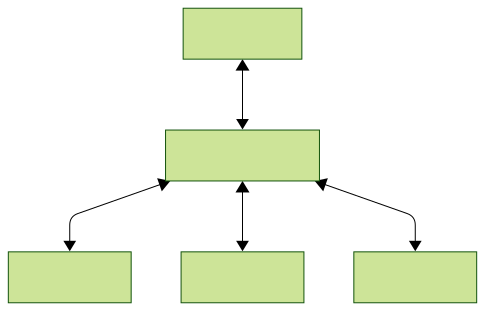
\includegraphics[width=\columnwidth]{images/architecture.png}
    \caption{Architecture Design for the Distributed File System. 
    The MetadataNode exposes the application API. The MetadataNode 
    and DataNodes communicate via the communication API.}
    \label{f:architecture}
\end{figure}

Figure \ref{f:architecture} visualizes the architecture of the simulator.
The workload communicates with the \code{MetadataNode} through the application
interface. The \code{MetadataNode} is connected to the various \code{DataNodes} and 
communicates through the communication interface.

The simulator simulates the "distributed" aspect of the file system by creating
different processes as data nodes which are created by the metadata node during
initialization. The different processes simulate running as different machines
by communicating through unix sockets.

\subsection{Application API}
\label{s:applicationapi}

The application API provides an interface for interacting with the distributed 
file system simulator. It exposes functions for initializing and shutting
down the file system, creating, reading, writing, and managing file system blocks.
The API is intended to be used by workloads that need to access or
manipulate file system data while abstracting the management.
The API can be categorized into three functional groups:
\begin{itemize}
    \item \textbf{Initialization and Cleanup}: Functions to start and stop the file
    system simulator. Involves creating the various data nodes and connecting to them.
    \item \textbf{File Management:} Functions for creating, locating, truncating, reading,
    and writing to files.
    \item \textbf{Block-level Operations:} Functions for directly reading and writing
    individual file blocks.
\end{itemize}

Below are the application interface functions that describe the operations that
the workload can interact with. The implementation of this API is currently simple,
as these functions call on metadata node functions. This limitation will be explained
later in the section.
 
The \code{init} function is used to initialize the simulator, it takes in a number
of datanodes to be used for the file system, as well as total file system capacity,
and a block allocation policy string. This function calls the metadata node
initialization.
\begin{lstlisting}
    init(int num_dns, size_t capacity, const char *policy_name)
\end{lstlisting}

The \code{exit} function is used to terminate the simulator. It takes a parameter, cleanup
which is used to clean up the data node directories or leave them as is. This
parameter is used so that the block distribution contents can be observed after
a workload has ended.
\begin{lstlisting}
    exit(int cleanup)
\end{lstlisting}

The \code{create\_file} function is used to create a file within the simulator. It takes
in a filename, a file size, and returns the file id of the file. This file id
is used to more easily identify a file within the file system.
\begin{lstlisting}
    create_file(const char *filename, size_t file_size, int *fid)
\end{lstlisting}

The \code{find\_file} function is used to find a file from its filename. This is a helper
function used to obtain a files file id given its name.
\begin{lstlisting}
    find_file(const char * filename, int * fid);
\end{lstlisting}

The \code{truncate\_file} function is used to change the size of a file given its file
id, with the new size of the file as a parameter. Depending on implementation
this may modify metadata only or modify actual file system blocks.
\begin{lstlisting}
    truncate_file(int fid, size_t new_size)
\end{lstlisting}

The \code{read\_file} function is used to read an entire files contents. The file id
is an input, and as an output, the file contents and file size are given.
\begin{lstlisting}
    read_file(int fid, void **buffer, size_t *file_size)
\end{lstlisting}

The \code{write\_file} function is used to write an entire files contents to the file
system. The file id, and buffer contents along with its size are inputs.
\begin{lstlisting}
    write_file(int fid, void *buffer, size_t buffer_size)
\end{lstlisting}

The \code{read\_block} function is used to read an individual block from a file given
its file id and the file index. The block contents are written to a buffer of that
size.
\begin{lstlisting}
    read_block(int fid, int file_index, void *buffer)
\end{lstlisting}

The \code{write\_block} function is used to write to an individual block from a file given
its file id and file index. The block contents are given as a buffer that will
be written to the file system.
\begin{lstlisting}
    write_block(int fid, int file_index, void * buffer)
\end{lstlisting}

The above functions serve as the public application API to the simulator. These
functions were used to investigate the performance of the simulator. Each operation
returns an enum of error or success codes which help identify if an operation 
was successful or not.

Currently, the application API does nothing more than call on metadata node functions.

\subsection{MetadataNode}
\label{s:metadatanode}

The \code{MetadataNode} is responsible for managing the data nodes, as well as 
keeping track of all of the file metadata and space for the file system. 
It has a few data structures that are used to keep track of this information 
and ensure communication between itself and the data nodes.

\begin{figure}[h]
    \centering
    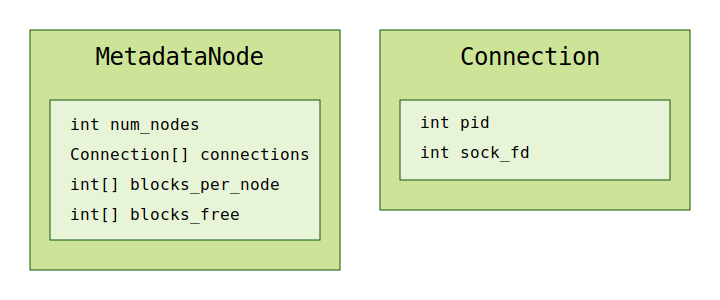
\includegraphics[width=\columnwidth]{images/metadata_struct1.png}
    \caption{\code{MetadataNode} structure tracking of the data nodes
    and connections.}
    \label{f:metadata_struct1}
\end{figure}

Figure \ref{f:metadata_struct1} shows the structure that the metadata node uses to
keep track of the nodes. It keeps track of the number of nodes, the connections
to the nodes, as well as a list of blocks per node, and the number of free blocks
each node has. The connections keep track of the process id, used only for clean
up, and the socked file descriptor which is used to communicate between the 
processes.

The \code{blocks\_per\_node} is used since the total file system capacity might
not be a clean multiple of the total number of nodes and some nodes may have more
blocks than others. For example, the case where there is 3 nodes but 4 blocks,
one node requires an extra block. The number of free blocks is also tracked
to avoid requests to allocate to a full node, which would return no space. 

\begin{figure}[h]
    \centering
    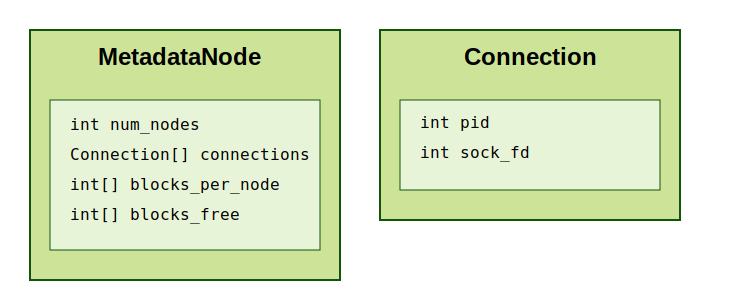
\includegraphics[width=\columnwidth]{images/metadata_struct2.png}
    \caption{\code{MetadataNode} structure tracking file system files and
    internal organization.}
    \label{f:metadata_struct2}
\end{figure}

Figure \ref{f:metadata_struct2} shows the structure that the metadata node uses
to keep track of the files in the file system and the internal organization.
The file system keeps track of the total capacity of the system, as well as
the total number of nodes in the system. It keeps track fo the number of
free blocks in the system. It uses a bitmap structure to keep track of which
blocks have been used.

It additionally keeps track of file metadata. It keeps track of the number of
files in the system. And keeps track of a file entry per file. The file entry
structure
contains its file id, the filename, and the number of blocks this file spans.
It additionally keeps track of a mapping from file blocks to logical blocks.
This file-to-block mapping helps us identify which file blocks map to which
logical blocks. The \code{block\_mapping} structure in the metadata node then maps logical blocks to
data nodes in the system, which help track where the logical blocks are.

In this implementation of the file system, to read a file the following 
structure is used:
\begin{enumerate}
    \item The \code{FileEntry} for the file is obtained by searching through
    the file entries. 
    \item For each file block index of the file entry, we use the \code{blocks} mapping
    to obtain the logical block this file block index maps to. Note that the file block
    corresponds to the index of the \code{blocks} array. The file block index corresponds
    to the order of the blocks within a file. For example, a file has file block indices 0, 1, 2, ...
    which map to blocks 245, 30, 49, ... in the global logical blocks.
    \item After obtaining the logical block index, the structure \code{block\_mapping}
    is used to obtain the corresponding data node which stores this logical block.
    The data node is found by indexing the \code{block\_mapping} structure at the
    logical block index.
    \item At this point, a request is made with the corresponding operation (a
    read) for that logical block stored in the involved data node. 
    \item Once the node returns, we add the result to the large buffer that all the
    reads are going into.
\end{enumerate}

% FIGURE HERE? EXPLAINING THE MAPPING?

Unlike GFS, the metadata node sits between the communication of the
workload/client and the data nodes. This is a limitation of the current design
since the metadata node becomes the bottleneck of the simulator. Every request
must be passed through the metadata node and every operation response must
also pass through the metadata node. To surpass this limitation, the
current design makes it such that the metadata node and workload are running
on the same process, and are thus simulated to run on the same machine.
This means that there is no actual communication between the workload and the
metadata node, the workload calls the metadata node API directly
through the application interface. This removes the metadata node from being the bottleneck 
of the application because there is no communication overhead between the
workload and metadata node. If the workload/client were to be uncoupled from the
metadata node, the application interface would now be responsible for sending and
receiving requests from the metadata node.
Below the metadata node interface alongside its implementation is described.

On initialization, the metadata node initializes the file system.
\begin{lstlisting}
metadatanode_init(int num_dns, size_t capacity, const char *policy_name)
\end{lstlisting}
The metadata node initializes the application with a specific file system size,
number of data nodes, and policy used for block allocation. This function is
responsible for creating each data node process, which is done by forking the
application and using sockets to communicate between each process. After creating
each data node, it connects to each by sending the \code{DN\_INIT} command to
each data node, which makes each data node initialize itself. After this function
returns, the file system is ready.

On exiting of the simulation, the metadata node can cleanup the system.
\begin{lstlisting}
metadatanode_exit(int cleanup)
\end{lstlisting}
Once this function is called, the metadata node commands each data node to shut
down. Given the parameter \code{cleanup}, it will order each data node to
clean up its files. The parameter can be used to inspect the imbalance and load
of each data node once the workload has finished.

The metadata node can create files with a given file size, and returns a file
id which identifies the file until closing.
\begin{lstlisting}
metadatanode_create_file(const char *filename, size_t file_size, int *fid)
\end{lstlisting}
The \code{fid} serves similar to an inode. 
There are various different implementations that were tested when calling this
function. Given the file size, the blocks could be allocated at this point, or
they could be allocated on write. The different implementations of when to
allocate blocks is discussed in a later section.

The metadata node is responsible for truncating a file.
\begin{lstlisting}
metadatanode_truncate_file(int fid, size_t new_size)
\end{lstlisting}
A file can be increased in size or decreased in size. On decrease, the metadata
node frees the relevant blocks based on the new size, it sends a \code{DN\_FREE\_BLOCK}
to each node for the block to free its memory. On increase, two things can happen,
either the blocks are allocated right away in each node, or just the metadata is 
allocated (similar to create file, blocks can be allocated on write).

The metadata node can read files through the file id.
\begin{lstlisting}
metadatanode_read_file(int fid, void **buffer, size_t *file_size)
\end{lstlisting}
The metadata node traverses through the file entries, and finds the 
corresponding file entry. It then loops through each file block, obtaining
the logical block corresponding to it. Then uses the block mapping to 
find the corresponding data node that stores it. It sends a \code{DN\_READ\_BLOCK}
command to the data node to read the corresponding block. It then stores the
block in the correct offset of the buffer. Once all of the blocks are processed,
it returns the buffer to the workload.

The metadata node can write to files through the file id.
\begin{lstlisting}
metadatanode_write_file(int fid, void *buffer, size_t buffer_size)
\end{lstlisting}
The metadata node traverses through the file entries, finds the corresponding
entry. Similarly to the previous function, it finds the corresponding logical
blocks, and data nodes that store them. It sends a \code{DN\_WRITE\_BLOCK} command
per block along with the block obtained from the offset in the buffer. 

The metadata node also exposes block level operations.
\begin{lstlisting}
metadatanode_read_block(int fid, int file_index, void *buffer)
metadatanode_write_block(int fid, int file_index, void * buffer)
\end{lstlisting}
These operations work in the same way as the file-level operations, except only
a single request is sent to the data node to read / write this file block.

\subsection{Communication API}
\label{s:communicationapi}

The communication API provides an interface for the communication between the
metadata node and the data nodes in the distributed file system. It exposes
functions for each type of node to send commands, receive commands,
and response to the commands.

The communication is two directional but initiated by the metadata node, meaning
the metadata node sends commands, and each data node responds.
There are eight types of commands that the metadata node can use to communicate with
the data node.
\begin{lstlisting}
    DN_INIT        | DN_EXIT
    DN_ALLOC_BLOCK | DN_FREE_BLOCK 
    DN_READ_BLOCK  | DN_WRITE_BLOCK
    DN_BATCH_READ  | DN_BATCH_WRITE
\end{lstlisting}
Each command is used alongside a buffer which sends the appropriate
information for that command. For example, \code{DN\_READ\_BLOCK} requires the
block index to be read and thus this needs to be sent to the data node as well.

\begin{figure}[h]
    \centering
    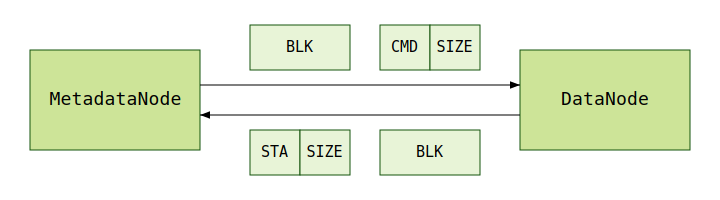
\includegraphics[width=\columnwidth]{images/communication.png}
    \caption{Packet communication structure between the \code{MetadataNode} and
    the \code{DataNode}.}
    \label{f:communication}
\end{figure}

Figure \ref{f:communication} presents the packet communication structure between
the metadata node and the data nodes. A request and response is serviced by
two packets each respectively. The first packet is static sized and contains
the command and the size of the second packet to be sent. The second packet
is variable sized and contains the necessary information involved with the
command. The second packet may contain information such as the block index to be
read, or the block index plus the block to be written, or in the case of batching,
various blocks and block indices. The response packets are organized in the same
way, except instead of a command being sent, a status code is sent back.

The metadata node sends commands through the following function.
\begin{lstlisting}
md_send_command(int sock_fd, DNCommand cmd, void *payload, size_t payload_size)
\end{lstlisting}
The function takes in the socket file descriptor (which data node connection to
send the command to), the command, a buffer with information for that command, 
and buffer size. As mentioned previously, the buffer (second packet) contains
information like the block and block index to be written to the data node. Or
just the block index to read. And in the case of batching, multiple blocks and
indices.

The metadata receives responses through the following function.
\begin{lstlisting}
md_recv_response(int sock_fd, DNStatus *status, void **payload, size_t *payload_size)
\end{lstlisting}
The function takes in a socket file descriptor of the node we are waiting on a message
as well as the status of the data node response, along with a potential packet.
If the data node fails, the metadata node is responsible for handling that error.
In this simulator, data node errors are only due to system errors such as out of memory
or IO errors when reading file blocks. Usually upon an error, the simulator shuts down.
Further considerations regarding reliability will be discussed in the further considerations
sections. If the data node is successful, the simulator can continue. The data node
can respond with a packet of information such as a block during a \code{DN\_READ\_BLOCK}.

The data node is responsible for receiving commands.
\begin{lstlisting}
dn_recv_command(int sock_fd, DNCommand *cmd, void **payload, size_t *payload_size)
\end{lstlisting}
The data node is constantly listening for commands in the service loop, and once
a command is received, it reads the command and payload expected for that command.
It then handles the appropriate command.

The data node sends responses to the metadata node once it has handled the command.
\begin{lstlisting}
dn_send_response(int sock_fd, DNStatus status, void *payload, size_t payload_size)
\end{lstlisting}
As mentioned previously, the simulator mostly sends success codes back to the
metadata node during normal execution. During succcess, the data node may send
blocks depending on the type of operation.

\subsection{DataNode}
\label{s:datanode}

The data nodes are responsible for storing the contents of each logical block
of the file system. Each datanode must keep track of a few data structures.

\begin{figure}[h]
    \centering
    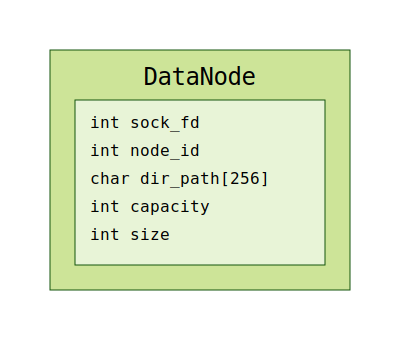
\includegraphics[width=0.65\columnwidth]{images/data_struct.png}
    \caption{\code{DataNode} structure for internal file tracking and connection.}
    \label{f:data_struct}
\end{figure}

The \code{DataNode} must keep track of its socket file descriptor to remain connected
to the \code{MetadataNode}. It additionally keeps track of its node id which
it uses to create a directory to store the file contents. Distributed file
systems tend to use the host file system to store files. In the case of this
simulator, the host file system is simulated by each nodes directory. Each node
only has access to the file blocks within their respective directory. It stores
the blocks in a file called \code{block\_\{id\}.dat}.

The \code{DataNode} additionally kept track of its capacity and current size.
These quantities are technically redundant as the metadata node keeps track
of each node's size and won't send blocks past its capacity. However as a safety
check these quantities prevent storage from overflowing in a node.

The datanode implementation will be described next.
The first function of the data node application is the service loop.
\begin{lstlisting}
datanode_service_loop(int sock_fd)
\end{lstlisting}
Once the metadata node creates each data node, each data node enters this loop.
The service loop consists of listening to the metadata node on a loop. Once
a command is received, the data node services the command and goes back to
listening for further commands. As mentioned previously, the data node can
receive the following commands:
\begin{lstlisting}
    DN_INIT        | DN_EXIT
    DN_ALLOC_BLOCK | DN_FREE_BLOCK 
    DN_READ_BLOCK  | DN_WRITE_BLOCK
    DN_BATCH_READ  | DN_BATCH_WRITE
\end{lstlisting}

The first command that the metadata node sends after creating each data node is
\code{DN\_INIT}. This command fills the purpose of initializing each data node.
\begin{lstlisting}
datanode_init(int sock_fd, void *payload, size_t payload_size)
\end{lstlisting}
This function initializes each data node with the node id and the capacity of this node. 
Since the simulator runs on one machine, the datanode creates a directory for 
itself where it will store the file blocks. Each data node only has access to its
own directory (identified by its node id).

The metadata node can send a command to write to a block through \code{DN\_WRITE\_BLOCK}.
\begin{lstlisting}
datanode_write_block(int block_index, void * buffer)
\end{lstlisting}
This function handles writing the buffer to a block with index \code{block\_index}.
As mentioned previously, the data node writes/overwrites the file to its directory.
Since data nodes store files of logical blocks of the file system, there are no
conflicts in overwriting files.

The metadata node can send a command to read a block through \code{DN\_READ\_BLOCK}.
\begin{lstlisting}
datanode_read_block(int block_index, void * buffer)
\end{lstlisting}
This function handles reading the file stored in the data nodes directory with the
relative block index, and write it to the buffer in preparation to send.

The metadata node can send a command to allocate a block through \code{DN\_ALLOC\_BLOCK}.
\begin{lstlisting}
datanode_alloc_block(int block_index)
\end{lstlisting}
This function handles allocating a block in the file system. The data node creates
an empty file for this block.

The metadata node can send a command to free a block through \code{DN\_FREE\_BLOCK}.
\begin{lstlisting}
datanode_free_block(int block_index)
\end{lstlisting}
This function handles freeing a block from the file system. The data node finds
the file and unlinks it to free its space from the file system.

The metadata node can send a command to exit the application through \code{DN\_EXIT}.
\begin{lstlisting}
datanode_exit(int cleanup, int * sock_fd)
\end{lstlisting}
On exit, each data node will clean up its resources. It will free the data node 
structure and free every file that is stored in its directory.

The metadata node can send a command to batch read a list of blocks stored in this 
data node through \code{DN\_BATCH\_READ}.
\begin{lstlisting}
datanode_batch_read(int *logical_blocks, int num_blocks, void *buffer)
\end{lstlisting}
The data node receives a list of logical blocks that are meant to be read. It
then reads each logical block and writes it to the buffer. The data node then
sends a success request back with the buffer.

The metadata node can send a command to batch write a list of blocks to be stored in
this data node through \code{DN\_BATCH\_WRITE}.
\begin{lstlisting}
datanode_batch_write(int *logical_blocks, int num_blocks, void *buffer)
\end{lstlisting}
The data node receives a list of logical blocks that are meant to be stored in
this data node. It writes each block from the buffer into its own \code{block\_\{id\}.dat}
file, and then returns a success code to the metadata node.

\subsection{Policies}
\label{s:policies}

The simulator was designed to be able to handle different block allocation
policies. Initially, the focus of the simulator was to study the block
allocation strategies and how they would affect the performance of the simulator.
However due to the sequential nature of the current simulator, the policies
perform quite similarly. Nevertheless, the policies implemented are listed below.

\subsubsection{Random}
\

Random allocation policy uses a random number to decide between the nodes.
However the metadata node does not attempt to allocate blocks on already full 
nodes as this would require extra communication requests. As mentioned previously,
the metadata node keeps track of the number of free blocks a node has. Thus
if the random number generated is to a full node, the allocation policy is attempted
again to generate another random number. If the number of attempts equal the number
of data nodes, the policy loops through the nodes in order to find an available
node. This is done since high number of attempts means the nodes are quite
full.

\subsubsection{Sequential}
\

Sequential allocation policy allocates on the same node starting from node 0
until the node becomes full. Then it allocates on the next node until it becomes
full. This process repeats. Thus in general, when a file that is created
it will likely be allocated on the same node, unless it is larger than the node's
capacity.

\subsubsection{Round Robin}
\

Round robin allocation policy allocates a block according to round robin. Round
robin initially starts with node 0 and allocates a block on each node before
allocating back on node 0.

\subsubsection{Least Loaded}
\

Least loaded allocation policy allocates a block on the least loaded node. This
allocation policy attempts to balance the overall load on each node.

\subsubsection{File Aware}
\

File aware allocation policy is a hybrid allocation policy which defines a
parameter \code{SMALL\_FILE\_THRESHOLD}. If the number of blocks to be 
allocated at the same time is lower than this threshold, the random policy is 
used, if the number of blocks to be allocated is larger, all of the blocks
are allocated on the least loaded node. This allocation policy was an attempt
to speed up the common case of small files.

The metadata node is responsible for using the allocation policy structure.
Each allocation policy exposes the same following functions:
\begin{lstlisting}
    int #policy#_init();
    int #policy#_alloc_block(AllocContext ctx, int *node_index);
    void #policy#_destroy();
\end{lstlisting}

% TODO: MORE HERE...

\subsection{File Distribution Experiments}

File distribution generators were created to perform different experiments for the
simulator. A file distribution generator returns a file size based on  pre-determined
workloads. For example, a generator might return files between 1-4 blocks large
and thus return a file size based on the number of blocks generated times the
block size for this workload run. The distributions are described below.

\begin{itemize}
    \item \code{UNIFORM\_SMALL}: Generates files that are uniformly randomly
    distributed between 1-4 blocks large.
    \item \code{UNIFORM\_LARGE}: Generates files that are uniformly randomly
    distributed between 8-16 blocks large.
    \item \code{WEB}: Generates files according to the following
    distribution: 70\% small (1-2 blocks), 20\% medium (4-8 blocks), 10\% large
    (16-32 blocks).
    \item \code{VIDEO}: Generates files uniformly randomly distributed betwen
    32-128 blocks large.
\end{itemize}

For an experiment, you can pick a specific file distribution generator to produce
files according to the above distributions. This lets you experiment with different
distributions and compare against block sizes, allocation policies, or
implementations of the simulator.

\subsection{Designs}

Various different designs where considered to investigate when blocks should
be allocated on each datanode and how to allocate the blocks. Each design is
described below.

\subsubsection{Preallocate on Create}
\

The first design considered was to pre-allocate all of the necessary blocks
for a file on file creation. During file creation, the file size is known since
it is a parameter. Thus the number of blocks for that file is known at this point.
At this point, the metadata node can allocate these blocks using the block 
allocation policy and send each involved data node a command to allocate a block.
Each data node will then create a file for that logical block and stored it in the
file system. 

This design was considered since at this point, the work of allocating blocks 
and creating the files is complete. And then on a write to the file, the files
would be populated without the overhead of creating the file. This design
was considered with speed in mind.

\subsubsection{Postallocate on Write}
\

The second design considered was to allocate (lazy allocate) necessary 
blocks on block/file writes instead of during file creation. During file 
creation, only the metadata is modified
in the metadata node and no communication to the data nodes is sent. On a block write,
the metadata node will send a write command to the involved node. The data
node will then be responsible for creating this file and storing the block contents.

The design was considered to solve two considerations. The first consideration is
of space, although it is uncommon to have holes in files, or empty blocks,
there might be cases where file blocks are allocated by have no actual
data inside (an example is when creating a large file, but only actually writing
a small amount). With the previous design, these blocks would be allocated on the
data node, thereby reducing the space of the data node with empty unused blocks.

The second consideration was speed. Consider the case where we create an empty
file with 4MB of data, but at this point have written nothing to the file.
If we try reading this file, in the previous design, the metadata node would
send requests to the datanodes to obtain all of the allocated blocks for the
file. However these blocks are empty and don't have any useful data inside. In
the new design, the metadata node can see the mapping for the file entry and see
that the logical blocks map to node -1. Meaning there is no mapping, which means
this block hasn't been allocated yet, and thus the metadata node does not need
to send any requests to the data nodes.

\subsubsection{Batch Operations per Node}
\

The third design considered was batching of blocks. In the two previous designs,
operations are heavily focused on blocks. Consider a round robin block allocation
of a file with 7 blocks and 2 data nodes. In this case we have the following
distribution of nodes outlined in Figure \ref{f:batch}.

\begin{figure}[h]
    \centering
    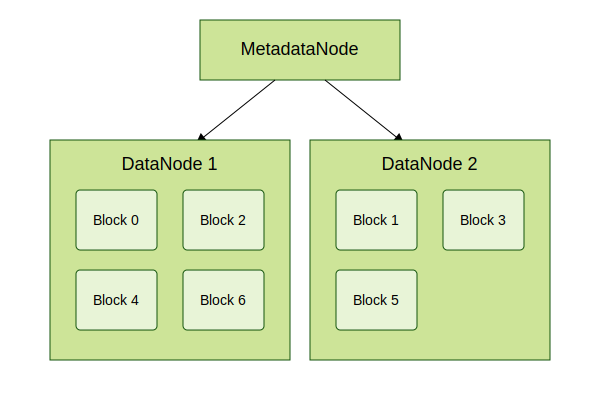
\includegraphics[width=\columnwidth]{images/batch.png}
    \caption{Distribution of blocks given 7 blocks for a file and round robin 
    allocation policy.}
    \label{f:batch}
\end{figure}

The distribution has 4 blocks on datanode 1 and 3 blocks on datanode 2. However
the order of the blocks relative to the file blocks make it so that they alternate
between the nodes.

In the previous implementations, the operations were done per block. Reading
a file involved looping through each file block in order, and sending a request 
to the mapped datanode for the block and waiting for a response. This 
resulted in the metadata node sending $O(\#\code{blocks})$ requests.

In this implementation, the focus was batching blocks for a file in a request. 
In the example above, datanode 1 has blocks 0, 2, 4, 6 for this file, which means
that we can send a single request to the datanode for those blocks, and obtain
a response with those 4 blocks. Similarly we send a request to datanode 2 for
the rest of the blocks. This means that we only send maximum $O(\#\code{datanodes})$ 
requests from the metadata node as the blocks from each data node are batched 
together in one request. The \code{FileEntry} structure must change to fit this
new way to process the blocks.

\begin{figure}[h]
    \centering
    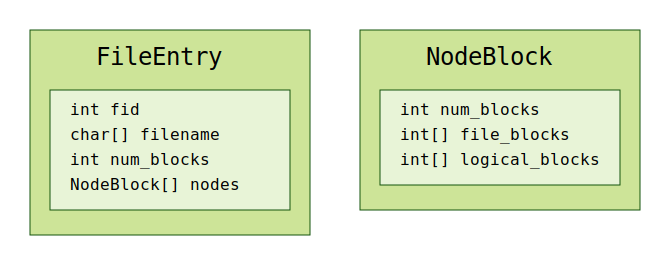
\includegraphics[width=\columnwidth]{images/metadata_struct3.png}
    \caption{Modified file entry structure to optimize for batching.}
    \label{f:metadata_struct3}
\end{figure}

Figure \ref{f:metadata_struct3} outlines the new \code{FileEntry} structure. I'll
first describe the new structure and then outline why its necessary.
In the new structure, file blocks are not stored as an array mapping from index
to logical blocks. In this case, for each data node in the system, the metadata
node keeps track of a \code{NodeBlock} structure. This structure keeps track of
the file blocks that a data node stores for this file (the index of the node block
indicates the data node index). The \code{NodeBlock} keeps track of the number of
blocks for this file it stores, and for each block it stores, the file block index
and the logical block that the file index maps to. To read a file, we do the 
following:
\begin{enumerate}
    \item The \code{FileEntry} for the file is obtained by searching through
    the file entries. The metadata node uses the global \code{num\_blocks} field
    to create a buffer that will contain the file that was read which will be
    returned to the application.
    \item For each node block (each data node), a request is sent to the data node
    with the list of logical blocks that it is storing.
    \item Once a response is received, the metadata node has a buffer equal to
    the number of blocks stored in the data node. It then uses the 
    \code{file\_blocks} field to map each block returned from the data node to its
    correct place in the large buffer.
\end{enumerate}

This structure is necessary because we want to optimize for batching, and thus
sending the list of logical blocks to the corresponding data node should be fast.
With the previous structure, it would require looping through the file blocks,
for each, using the block mapping to obtain the logical block, and group it
to the corresponding array for each data node. This would increase processing
before sending the request.

However, this new structure adds complexity in keeping track of blocks in the file entry. 
Block-level queries to read / write a single block of a file requires more processing
as now we need to search through the node blocks to obtain which data node stores
this file block to send a request to. 

A compromise might be to combine the structures. Keep the previous structure which
was optimized for block-level queries, and add the new structure to optimize for
batch-level queries. This however adds redundancy which would increase the
metadata size overhead.

There is an additional tradeoff to consider. As block sizes get bigger, the 
number of blocks for a file get smaller. If we consider a 1MB file with 64KB 
block size, that gives us 16 blocks, and if the number of data nodes is at 
least this, there is no benefit to batching. Thus batching and larger block
sizes work 

This is however, extremely workload dependent as it will depend
on how large the files are in the workload, and how many data nodes there are.
However this gives us an indication that tuning the block size to fit the
workload can give us the best benefit for batching. And that in some cases (very
small files) batching may be unnecessary.
